\label{sec:problem_form}

Consider $N$ agents interacting with an environment that is modeled as an MDP with transition probabilities $\mathbb{P}\left(S_{t+1}\mid S_{t},A_{t}\right)$. For each time index $t=0,1,2,\ldots$, random variables $S_t=(S_t^1,\ldots,S_t^N)$ and $A_t=(A_t^1,\ldots,A_t^N)$ collect the states $S_t^n\in \mathcal S$ and actions $A_t^n\in \mathcal A$ for all agents. The team receives a vector of rewards $r(S_t)\in \mathbb R^M$ associated with $M$ different tasks that must be collectively satisfied. We consider a family of assignment problems in which the agents must persistently cover $M$ regions of the state space denoted by $\mathcal{S}_m\subset\mathcal{S}$ with $m=1,\ldots,M$. Thus, each reward is given by
%
\begin{equation}\label{eqn_patrolling_reward}
%    r_m(S_t,A_t) = \max_{n=1,\ldots,N} \mathds{1}[S_{tn}\in \mathcal{S}_m]
    \left(r(S_t)\right)_m = \max_{n=1,\ldots,N} \mathds{1}[S_t^n\in \mathcal{S}_m],
\end{equation}
where  $\left(r\right)_m$ represents the $m$-th element of vector $r$,  with the index function defined as
    $\mathds{1}[S_t^n\in \mathcal{S}_m]=1 $ if $  S_t^n\in \mathcal{S}_m$ and zero otherwise. %,
%
Each region $\mathcal S_m$ must be covered by the agents a fraction of the time. Hence, we set the requirements as a vector $c\in[0,1]^M$ of $M$ thresholds on the average rewards, and formulate a Markov decision problem with constraints
\begin{equation}\label{eqn_ideal_V}
    V(\pi):= \lim_{T\to \infty}\frac{1}{T} \mathbb E_{S_t, A_t\sim \pi} \left [ \sum_{t=0}^{T-1} r(S_t) \right ] \geq c,
    \end{equation}
%
with the inequality being component-wise. The expectation is taken over the transition probabilities and the probability distribution defining the control policy $\pi(A_t|S_t)$  of the actions of all agents given their states.

A task reward can be incorporated to establish an optimization objective. This can be useful to set a secondary goal, such as minimizing energy consumption in a multi-robot application like the one presented in Example \ref{example} below. However, in the following, we will set the objective to zero and focus on our primary goal of satisfying the specifications.

Hence, the feasibility problem we aim to solve is
%
\begin{align}\label{eqn_crl}
P^\star = &\; \max_{{\pi}} 0\\*
\textrm{s. to} &\; \lim_{T\to \infty}\frac{1}{T} \mathbb E_{S_t, A_t\sim \pi} \left [ \sum_{t=0}^{T-1} r(S_t) \right ] \geq c.\notag 
\end{align}
%
To illustrate the practical use of this problem formulation, we include the following example, which we will explore further in the experiments of Section \ref{sec_numerical}.

\begin{example}\label{example}
Consider a team of $N$ robots that is required to monitor $M>N$ areas,  visiting areas $\mathcal S_1,\ldots,\mathcal S_M$ during fractions of time given by  $c\in [0,1]^M$. These conflicting requirements may not be achievable by a single robot, particularly when the aggregate thresholds are greater than one, i.e., $\left\|c\right\|_1>1$, and not even by multiple robots acting independently following the same optimal single-agent policy. Coordination is thus essential, for which robots can form an ad-hoc communication network. 
\end{example}
%



We aim to solve \eqref{eqn_crl} in a coordinated distributed fashion, in a scenario in which agents do not have access to the whole system state but can only observe their own state $S_t^n$. Once deployed, agents will not share their locations. Instead, we will develop a light gossip protocol for agents to exchange \emph{single-bit messages} with their neighbors (Section \ref{sec_online_execution}) over an ad-hoc communication network adhering to the stochastic graph model in \cite{Nedic2017Achieving}.  This graph model considers a time domain $\mathcal T \subset \mathbb N$ and a set of nodes $\mathcal V=\{1,\ldots,N\}$ representing the agents. Then, $\mathcal G = \mathcal G(\mathcal V,\mathcal E,\mathcal T, w_G)$ defines a stochastic graph where edges are sampled from a static underlying graph $G = (\mathcal V, \mathcal E)$. This \textit{footprint} graph $G$ indicates pairs of agents that could have connectivity at some point in time. In this model,  $G$ is assumed to be connected, but it is noteworthy that this does not necessarily imply that $\mathcal G$ is connected. Indeed, $\mathcal G$ could be disconnected at all times. Accordingly, the \textit{presence} function $w_G: \mathcal E \times \mathcal T \to \{0,1\}$ is included to indicate if an edge is present at a given time.
%
We will consider a probabilistic model in which the presence of an edge 
$e^{(n,n^\prime)} \in\mathcal{E}$ 
between two agents    $n,n^\prime \in \mathcal{V}$  at time $t$ is modeled as a Bernoulli random variable with probability $p$, i.e., 
%
\begin{align}
w_G\left(n,n^\prime,t\right)& \text{ are i.i.d. }  \text{Bernoulli}(p).\label{eqn_graph_model}
\end{align} 
Edges are independent of each other, as it is also the activation of an edge across time.   Figure \ref{fig:gossip_stochastic} illustrates the communication graph for the monitoring problem in Example \ref{example}.

\begin{figure}[t]
    \centering
    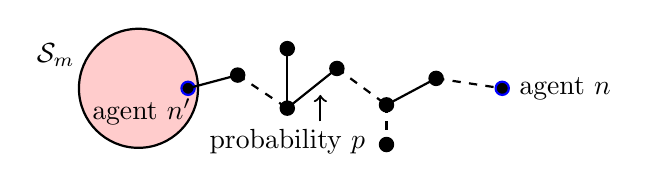
\begin{tikzpicture}[scale=0.42]

    % Main zones
    \filldraw[color=black, fill=red!20, thick] (0,0) circle (1.8cm); % Smaller zone around agent i
    \filldraw[color=blue, fill=black, thick] (1.5,0) circle (0.2); % Agent i
    \filldraw[color=blue, fill=black, thick] (11,0) circle (0.2); % Agent n

    % Intermediate nodes on a zigzag path between i and n
    \filldraw[color=black, fill=black, thick] (3,0.4) circle (0.2);    % Node 1 (slightly above)
    \filldraw[color=black, fill=black, thick] (4.5,-0.6) circle (0.2); % Node 2 (slightly below)
    \filldraw[color=black, fill=black, thick] (6,0.6) circle (0.2);    % Node 3 (slightly above)
    \filldraw[color=black, fill=black, thick] (7.5,-0.5) circle (0.2); % Node 4 (slightly below)
    \filldraw[color=black, fill=black, thick] (9,0.3) circle (0.2);    % Node 5 (slightly above)

    % Dotted line segments connecting nodes from agent i to agent n
    \draw[color=black, thick] (1.5,0) -- (3,0.4);
    \draw[color=black, thick,dashed] (3,0.4) -- (4.5,-0.6);
    \draw[color=black, thick] (4.5,-0.6) -- (6,0.6);
    \draw[color=black, thick, dashed] (6,0.6) -- (7.5,-0.5);
    \draw[color=black, thick] (7.5,-0.5) -- (9,0.3);
    \draw[color=black, thick,dashed] (9,0.3) -- (11,0);

    % Branching nodes
    \filldraw[color=black, fill=black, thick] (4.5,1.2) circle (0.2); % Branch above
    \draw[color=black, thick] (4.5,-0.6) -- (4.5,1.2);

    \filldraw[color=black, fill=black, thick] (7.5,-1.7) circle (0.2); % Branch below
    \draw[color=black, thick, dashed] (7.5,-0.5) -- (7.5,-1.7);

    % Arrow pointing to a dotted line segment with probability label
    \draw[->, thick] (5.5,-1.) -- (5.5,-0.2);
    \draw node at (4.5,-1.6) {probability $p$};

    % Labels
    \draw node at (-2.5,1) {$\mathcal S_m$};
    \draw node at (0.1,-0.7) {agent $n'$};
    \draw node at (12.9,0) {agent $n$};

\end{tikzpicture}
    \caption{\label{fig:gossip_stochastic}Agent $n$ must receive the information that agent $n^\prime$ is in zone $\mathcal S_m$ across the communication graph. Agents \( n \in \mathcal{V} = \{1, \dots, N\} \) are nodes in the stochastic graph \( \mathcal{G}(\mathcal{V}, \mathcal{E}, p) \), where solid and dashed lines represent the presence or absence of an edge, respectively, at a particular time. If an edge is present, the two nodes connected to the edge can exchange information. Otherwise, the two neighboring agents must wait for a future time in which the edge is present. }
\end{figure}

